\chapter{Using Recurrent Neural Networks for Slot Filling in Spoken Language Understanding \label{chap:rnn}}

\section{Introduction}

The term "spoken language understanding" (SLU) refers to the targeted
understanding of human speech directed at machines \citep{rnn1}. The goal of such
"targeted" understanding is to convert the recognition of user input, $S_i$, into
a task-specific semantic representation of the user's intention, $U_i$ at each
turn. The dialog manager then interprets $U_i$ and decides on the most
appropriate system action, $A_i$, exploiting semantic context, user specific
meta-information, such as geo-location and personal preferences, and other
contextual information.

The semantic parsing of input utterances in SLU typically consists of three
tasks: domain detection, intent determination, and slot filling. Originating
from call routing systems, the domain detection and intent determination tasks
are typically treated as semantic utterance classification problems \citep{rnn2,rnn3,rnn4,rnn30}.
Slot filling is typically treated as a sequence classification problem in which
contiguous sequences of words are assigned semantic class labels.
\citep{rnn5,rnn7,rnn31,rnn32,rnn33,rnn34,rnn40,rnn55}. 

In this paper, following the success of deep learning methods for semantic
utterance classification such as domain detection \citep{rnn30} and intent determination
\citep{rnn13,rnn39,rnn50}, we focus on applying deep learning methods for slot filling.
Standard approaches to solving the slot filling problem include generative
models, such as HMM/CFG composite models \citep{rnn31,rnn5,rnn53}, hidden vector state (HVS)
model \citep{rnn33}, and discriminative or conditional models such as conditional random
fields (CRFs) \citep{rnn6, rnn7, rnn32, rnn34, rnn40, rnn51, rnn54} and support vector machines (SVMs) \citep{rnn52}.
Despite many years of research, the slot filling task in SLU is still a
challenging problem, and this has motivated the recent application of a number
of very successful continuous-space, neural net, and deep learning approaches,
e.g. \citep{rnn13,rnn15,rnn24,rnn30,rnn56}. 

In light of the recent success of these methods, especially the success of RNNs
in language modeling \citep{rnn22, rnn23} and in some preliminary SLU experiments
\citep{rnn15,rnn24,rnn30,rnn56}, in this paper we carry out an in-depth investigation of RNNs for
the slot filling task of SLU. In this work, we implemented and compared several
important RNN architectures, including the Elman-type networks \citep{rnn16},
Jordan-type networks \citep{rnn17} and their variations. To make the results easy to
reproduce and rigorously comparable, we implemented these models using the
common Theano neural network toolkit \citep{rnn25} and evaluated them on the standard
ATIS (Airline Travel Information Systems) benchmark. We also compared our
results to a baseline using conditional random fields (CRF). Our results show
that on the ATIS task, both Elman-type networks and Jordan-type networks
outperform the CRF baseline substantially, and a bi-directional Jordan-type
network that takes into account both past and future dependencies among slots
works best.

In the next section, we formally define the semantic utterance
classification problem along with the slot filling task and present the
related work. In Section \ref{sec:deepreview}, we propose a brief review of deep learning
for slot filling. Section \ref{sec:rnnsf} more specifically describes our approach of
RNN architectures for slot filling. We describe sequence level
optimization and decoding methods in Section \ref{sec:slod}. Experimental results
are summarized and discussed in section \ref{sec:exp}.

\section{Slot Filling in Spoken Language Understanding}
\label{sec:sfslu}

A major task in spoken language understanding in goal-oriented human-machine
conversational understanding systems is to automatically extract semantic
concepts, or to fill in a set of arguments or "slots" embedded in a semantic
frame, in order to achieve a goal in a human-machine dialogue. 

An example sentence is provided in Table~\ref{fig:iob}, with domain, intent, and slot/concept
annotations illustrated, along with typical domain-independent named entities.
This example follows the popular in/out/begin (IOB) representation, where {\it
Bostoi} and {\it New York} are the departure and arrival cities specified as
the slot values in the user's utterance, respectively.

\begin{table}
\begin{tabular}{|c|c|c|c|c|c|c|c|c|}
\hline
{\bf Sentence} & show & flights & from & Boston & to & New & York & today \\
\hline
{\bf Slots/Concepts} & O & O & O & B-dept & O & B-arr & I-arr & B-date \\
\hline
{\bf Named Entity} & O & O & O & B-city & O & B-city & I-city & O \\
\hline
{\bf Intent} & \multicolumn{8}{c|}{Find\_Flight} \\
\hline
{\bf Domain} & \multicolumn{8}{c|}{Airline Travel} \\
\hline
\end{tabular}
\caption[IOB representation]{ATIS utterance example IOB representation}
\label{fig:iob}
\end{table}

While the concept of using semantic frames (templates) is motivated by the case
frames of the artificial intelligence area, the slots are very specific to the
target domain and finding values of properties from automatically recognized
spoken utterances may suffer from automatic speech recognition errors and poor
modeling of natural language variability in expressing the same concept. For
these reasons, spoken language understanding researchers employed statistical
methods. These approaches include generative models such as hidden Markov
models, discriminative classification methods such as CRFs, knowledge-based
methods, and probabilistic context free grammars. A detailed survey of these
earlier approaches can be found in \citep{rnn7}.

For the slot filling task, the input is the sentence consisting of a sequence
of words, $L$, and the output is a sequence of slot/concept IDs, $S$, one for each
word. In the statistical SLU systems, the task is often formalized as a pattern
recognition problem:  Given the word sequence $L$, the goal of SLU is to find the
semantic representation of the slot sequence $S$ that has the maximum {\it a
posteriori} probability $P(S | L)$. 

In the generative model framework, the Bayes rule is applied:

\begin{equation}
\hat{S} = \textrm{arg}\max_{S} P(S\vert L) = \textrm{arg}\max_{S} P(L \vert S) P (S)
\end{equation}

The objective function of a generative model is then to maximize the joint
probability $P(L | S)P(S) = P(L, S)$ given a training sample of $L$, and its semantic
annotation, $S$.

The first generative model, used by both the AT\&T CHRONUS system \citep{rnn31} and the
BBN Hidden Understanding Model (HUM) \citep{rnn35}, assumes a deterministic one-to-one
correspondence between model states and the segments, i.e., there is only one
segment per state, and the order of the segments follows that of the states.  

As another extension, in the Hidden Vector State model the states in the
Markov chain representation encode all the structure information about the
tree using stacks, so the semantic tree structure (excluding words) can be
reconstructed from the hidden vector state sequence. The model imposes a hard
limit on the maximum depth of the stack, so the number of the states becomes
finite, and the prior model becomes the Markov chain in an HMM \citep{rnn33}.

Recently, discriminative methods have become more popular. One of the most
successful approaches for slot filling is the conditional random field (CRF)
\citep{rnn6} and its variants. Given the input word sequence $L_1^N=l_1,\dots,l_N$, the
linear-chain CRF models the conditional probability of a concept/slot sequence
$S_1^N=s_1,\dots,s_N$ as follows:

\begin{equation}
P(S_{1}^{N}\vert L_{1}^{N}) = \frac{1}{Z}\prod_{t=1}^{N}\exp{H(s_{t-1}, s_{t}, l_{t-d}^{t+d}})
\label{eq:crf1}
\end{equation}

where

\begin{equation}
H(s_{t-1}, s_{t}, l_{t-d}^{t+d}) = \sum_{m=1}^{M}\lambda_{m}h_{m}(s_{t-1}, s_{t}, l_{t-d}^{t+d})
\label{eq:crf2}
\end{equation}

and $h_m (s_{t-1},s_t,l_{t-d}^{t+d})$ are features extracted from the current and
previous states $s_t$ and $s_{t-1}$, plus a window of words around the current word
$l_t$, with a window size of $2d+1$.

CRFs have first been used for slot filling by \citep{rnn33}. CRF
models have been shown to outperform conventional generative models. Other
discriminative methods such as the semantic tuple classifier based on SVMs \citep{rnn36}
has the same main idea of semantic classification trees as used by the Chanel
system \citep{rnn37}, where local probability functions are used, i.e., each phrase is
separately considered to be a slot given features. More formally,

\begin{equation}
P(S_{1}^{N}\vert L_{1}^{N}) = \prod_{t=1}^{N} P(s_{t} \vert s_{1}^{t-1}, L_{1}^{N})
\end{equation}

These methods treat the classification algorithm as a black box implementation
of linear or log-linear approaches but require good feature engineering. As
discussed in \citep{rnn57,rnn13}, one promising direction with deep learning architectures
is integrating both feature design and classification into the learning
procedure.

\section{Deep Learning Review}
\label{sec:deepreview}

In comparison to the above described techniques, deep learning uses many layers
of neural networks \citep{rnn57}. It has made strong impacts on applications ranging
from automatic speech recognition \citep{rnn8} to image recognition \citep{rnn10}. 

A distinguishing feature of NLP applications of deep learning is that inputs
are symbols from a large vocabulary, which led the initial work on neural
language modeling \citep{rnn26} to suggest map words to a learned distributed
representation either in the input or output layers (or both), with those
embeddings learned jointly with the task. Following this principle, a variety
of neural net architectures and training approaches have been successfully
applied \citep{rnn11,rnn13,rnn20,rnn22,rnn23,rnn39,rnn49,rnn58,rnn59,rnn60,rnn61}. Particularly, RNNs \citep{rnn22,rnn23,rnn49} are
also widely used in NLP. One can represent an input symbol as a one-hot vector,
i.e., containing zeros except for one component equal to one, and this weight
vector is considered as a low-dimensional continuous valued vector
representation of the original input, called word embedding. Critically, in
this vector space, similar words that have occurred syntactically and
semantically tend to be placed by the learning procedure close to each other,
and relationships between words are preserved. Thus, adjusting the model
parameters to increase the objective function for a training example which
involves a particular word tends to improve performances for similar words in
similar context, thereby greatly improving generalization and addressing the
curse-of-dimensionality obstacle faced with traditional n-gram non-parametric
models \citep{rnn26}.

One way of building a deep model for slot filling is to stack several neural
network layers on top of each other. This approach was taken in \citep{rnn27}, which
used deep belief networks (DBNs), and showed superior results to a CRF baseline
on ATIS. The DBNs were built with a stack of Restricted Boltzmann Machines
(RBMs) \citep{rnn12}. The RBM layers were pre-trained to initialize the weights. Then
the well-known back-propagation algorithm was used to fine-tune the weights of
the deep network in a discriminative fashion. Once the individual local models
are trained, Viterbi decoding is carried out to find the best slot sequence
given the sequence of words. 

In contrast to using DBNs, we propose recurrent neural networks (RNNs). The
basic RNNs used in language modeling read an input word and predict the next
word. For SLU, these models are modified to take a word and possibly other
features as input, and to output a slot value for each word. We will describe
RNNs in detail in the following section. 

\section{Recurrent Neural Networks for Slot-Filling}
\label{sec:rnnsf}

We provide here a description of the RNN models used for the slot filling task. 

\subsection{Words Embeddings}

The main input to a RNN is a one-hot representation of the next input word. The
first-layer weight matrix defines a vector of weights for each word, whose
dimensionality is equal to the size of the hidden layer (Fig.~\ref{fig:rnn}) - typically a
few hundred. This provides a continuous-space representation for each word.
These neural word embeddings \citep{rnn26} may be trained a-priori on external data such
as the Wikipedia, with a variety of models ranging from shallow neural networks
\citep{rnn21} to convolutional neural networks \citep{rnn20} and RNNs \citep{rnn22}. Such word embeddings
actually present interesting properties \citep{rnn23} and tend to cluster \citep{rnn20} when
their semantics are similar.

\begin{figure}[t]
\begin{center}
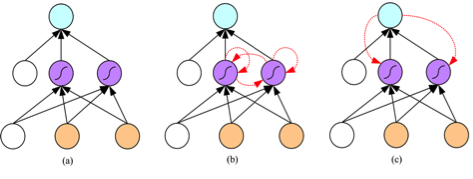
\includegraphics[width=.8\linewidth]{article4/images/rnn.png}
\caption[Forward and Recurrent Neural Networks Architectures]{\label{fig:rnn} Three different types of neural networks 
(a) Feed-forward NN; (b) Elman-RNN; (c) Jordan-RNN}
\vspace{-0.2in}
\end{center}
\vspace*{-1mm}
\end{figure}


While \citep{rnn15, rnn24} suggest initializing the embedding vectors with unsupervised
learned features and then fine-tune it on the task of interest, we found that
directly learning the embedding vectors initialized from random values led to
the same performance on the ATIS dataset, when using the SENNA
\footnote{http://ml.nec-labs.com/senna/} word embeddings. While this behavior
seems very specific to ATIS, we considered extensive experiments about
different unsupervised initialization techniques out of the scope of this
paper. Word embeddings were initialized randomly in our experiments.

\subsection{Context Word Window}

Before considering any temporal feedback, one can start with a context word
window as input for the model. It allows one to capture short-term temporal
dependencies given the words surrounding the word of interest. Given $d_e$ the
dimension of the word embedding and $|V|$ the size of the vocabulary, we
construct the d-context word window as the ordered concatenation of $2d+1$ word
embedding vectors, i.e. $d$ previous word followed by the word of interest and $d$
next words, with the following dot product:

\begin{equation}
C_{d}(l_{i-d}^{i+d}) = \tilde{E}\tilde{l}_{i-d}^{i+d}\in\mathbb{R}^{d_{e} (2d+1)}
\end{equation}

where $\tilde{E}$ corresponds to the embedding matrix
$E\in\mathcal{M}_{d_e\times|V|}(\mathbb{R})$ replicated vertically $2d+1$ times
and $\tilde{l}_{i-d}^{i+d}= [
\tilde{l}_{i-d},\dots,\tilde{l}_i,\dots,\tilde{l}_{i+d}]^T\in\mathbb{R}^{|V|(2d+1)}$
corresponds to the concatenation of one-hot word index vectors $\tilde{l}_i$.

\begin{equation}
\tilde{l}_{i}(\textrm{"flight"}) =
\begin{bmatrix}
0\\
\vdots\\
1\\
\vdots\\
0\\
\end{bmatrix} 
\leftarrow \textrm{The index of word "flight" in the vocabulary}
\end{equation}

In this window approach, one might wonder how to build a $d$-context window for
the first/last words of the sentence. We work around this border effect problem
by padding the beginning and the end of sentences $d$ times with a special token.
In Table~\ref{fig:cwmap}, we depict an example of building a context window of size $3$ around the
word "from":

\begin{table}
\centering
\begin{tabular}{c}
$l(t)=[$flights, {\bf from}, Boston $]$ \\
"from" $\rightarrow l_{\textrm{from}}\in\mathbb{R}^{d_e}$ \\
$l(t)\rightarrow C_{3}(t)=[l_{\textrm{flights}}, l_{\textrm{{\bf from}}}, l_{\textrm{Boston}}]$
\end{tabular}
\caption[Context Window Mapping]{
\label{fig:cwmap}
Context window mapping example}
\end{table}

In this example, $l(t)$ is a $3$-word context window around the $t$-th word
"from".  $l_{\textrm{from}}$ corresponds to the appropriate line in the
embedding matrix $E$ mapping the word "from" to its word embedding. Finally,
$C_3 (t)$ gives the ordered concatenated word embeddings vector for the
sequence of words in $l(t)$.

\subsection{Elman, Jordan and Hybrid architectures}

As in \citep{rnn15}, we describe here the two most common RNN architectures in the
literature: the Elman \citep{rnn16} and Jordan \citep{rnn17} models. The architectures of these
models are illustrated in Fig.~\ref{fig:rnn}.

In contrast with classic feed-forward neural networks, the Elman neural network
keeps track of the previous hidden layer states through its recurrent
connections. Hence, the hidden layer at time $t$ can be viewed as a state
summarizing past inputs along with the current input. Mathematically, Elman
dynamics with $d_h$ hidden nodes at each of the $H$ hidden layers are depicted
below:

\begin{equation}
h^{(1)}(t) = f(U^{(1)}C_{d}(l_{t-d}^{t+d})+U^{'(1)}h^{(1)}(t-1))
\end{equation}

\begin{equation}
h^{(n+1)}(t) = f(U^{(n+1)}h^{(n)}(t) + U^{'(n+1)}h^{(n+1)}(t-1))
\end{equation}


where we used the non-linear sigmoid function applied element wise for the
hidden layer $f(x)=1/(1+\exp{-x})$ and $h^{(i)} (0)\in\mathbb{R}^{d_h}$ are parameter vectors
to be learned. The superscript denotes the depth of the hidden layers and $U^{'}$
represents the recurrent weights connection. The posterior probabilities of the
classifier for each class are then given by the softmax function applied to the
hidden state:

\begin{equation}
P(y(t) = i \vert l_{0}^{t+d}) = \frac{\exp{\sum_{j=1}^{d_{h}}}V_{i,j}h_{j}^{(H)}(t)}{\sum_{i=1}^{N}\exp{\sum_{j=1}^{d_{h}}}V_{i,j}h_{j}^{(H)}(t)}
\end{equation}

Where $V$ correspond to the weights of the softmax top layer. 

The learning part then consists of tuning the parameters $\theta=\{ E, h^{(1)}
(0), U^{(1)}, \\ U^{'(1)},\dots,h^{(H)} (0), U^{(H)}, U^{'(H)} ,V \}$   of the RNN with $N$
output classes. Precisely, the matrix shapes are $U^{(1)}\in\mathcal{M}_{d_h\times d_e (2d+1)}
(\mathbb{R})$~;~ $U^{'(1)},\dots,U^{(H)}, U^{'(H)}\in\mathcal{M}_{d_h\times d_h} (\mathbb{R})$ and $V\in\mathcal{M}_{N\times d_h}(\mathbb{R})$. For
training, we use stochastic gradient descent, with the parameters being updated
after computing the gradient for each one of the sentences in our training set
$\mathcal{D}$, towards minimizing the negative log-likelihood. Note that a sentence is
considered as a tuple of words and a tuple of slots:

\begin{equation}
\mathcal{L}(\theta) = \sum_{(S,W)\in\mathcal{D}} \sum_{t=1}^{T}\log P_{\theta}(s_{t}\vert l_{0}^{t+d})
\end{equation}

Note that the length $T$ of each sentence can vary among the training samples and
the context word window size $d$ is a hyper-parameter.  

The Jordan RNN is similar to the Elman-type network except that the recurrent
connections take their input from the output posterior probabilities:

\begin{equation}
h(t) = f(UC_{d}(l^{t+d}_{t-d})+ U^{'}P(y(t-1)))
\end{equation}


where $U^{'}\in\mathcal{M}_{d_h\times N} (\mathbb{R})$ and
$P(y(0))\in\mathbb{R}^{N}$ are additional parameters to tune. As pointed out in
\citep{rnn15}, three different options can be considered for the feedback connections:
(a) $P(y(t-1))$, (b) a one-hot vector with an active bit for $\textrm{arg}
\max_i P_i(y(t-1))$ or even (c) the ground truth label for training.
Empirically \citep{rnn15}, none of these options significantly outperformed all others.  

In this work, we focused on the Elman-type, Jordan-type and hybrid versions of
RNNs. The hybrid version corresponds to a combination of the recurrences from
the Jordan and the Elman models:

\begin{equation}
h(t) = f(UC_{d}(l^{t+d}_{t-d})+ U^{'}P(y(t-1)) + U^{*}h(t-1))
\end{equation}

\subsection{Forward, Backward and Bidirectionnal variants}

In slot filling, useful information can be extracted from the future and we do
not necessarily have to process the sequence online in a single forward pass.
It is also possible to take into account future information with a single
backward pass but still, this approach uses only partial information available.
A more appealing model would consider both past and future information at the
same time: it corresponds to the bi-directional Elman \citep{rnn18, rnn19} or Jordan \citep{rnn15}
RNN.


We describe the bidirectional variant only for the first layer since it is
straightforward to build upper layers as we did previously for the Elman RNN.
First, we define the forward $\overrightarrow{h}(t)$ and the backward
$\overleftarrow{h}(t)$ hidden layers:

\begin{equation}
\overrightarrow{h}(t) = f(\overrightarrow{U}C_{d}(l^{t+d}_{t-d})+ \overrightarrow{U}^{'}\overrightarrow{h}(t-1))
\end{equation}
\begin{equation}
\overleftarrow{h}(t) = f(\overleftarrow{U}C_{d}(l^{t+d}_{t-d})+ \overleftarrow{U}^{'}\overleftarrow{h}(t-1))
\end{equation}

where $\overrightarrow{U}$ corresponds to the weights for the forward pass
and $\overleftarrow{U}$ for the backward pass. The superscript $U^{'}$
corresponds to the recurrent weights.  The bidirectional hidden layer $ \dvec
h (t)$ then takes as input the forward and backward hidden layers:


\begin{equation}
\dvec h (t) = f(BC_{d}(l^{t+d}_{t-d})+B^{'}\overrightarrow{h}(t-1)+ B^{*}\overleftarrow{h}(t+1))
\end{equation}

where $B$ are the weights for the context window input, $B^{'}$ projects the
forward pass hidden layer of the previous time step (past), and $B^{*}$ the
backward hidden layer of the next time step (future).


\section{Sequence Level Optimization and Decoding} \label{sec:slod}

The previous architectures are optimized based on a tag-by-tag likelihood as
opposed to a sequence-level objective function. In common with Maximum Entropy
Markov Model (MEMM) \citep{rnn28} models, the RNNs produce a sequence of
locally-normalized output distributions, one for each word position. Thus, it
can suffer from the same label bias \citep{rnn6} problem. To ameliorate these problems,
we propose two methods: Viterbi decoding with slot language models and
recurrent CRF.

\subsection{Slot Langage Models}

As just mentioned, one advantage of CRF models over RNN models is that it is
performing global sequence optimization using tag level features. In order to
approximate this behavior, and optimize the sentence level tag sequence, we
explicitly applied the Viterbi \citep{rnn40} algorithm. To this end, a second order
Markov model has been formed, using the slot tags, $s_{i}\in S$ as states, where the
state transition probabilities, $P_{(LM)}  (s_{i}\vert s_{j} )$ are obtained using a trigram
tag language model $(LM)$. The tag level posterior probabilities obtained from
the RNN were used when computing the state observation likelihoods.

\begin{align*}
\centering
\hat{S} & =  \textrm{arg}\max_{S} P(S\vert L) \\
& =  \textrm{arg}\max_{S} P_{(LM)}(S)^{\alpha}\times P(L \vert S)\\
& =  \textrm{arg}\max_{S} P_{(LM)}(S)^{\alpha}\times \prod_{t} \frac{P_{\textrm{RecNN}}(s_{t}\vert l_{t})}{P(s_{t})}
\end{align*}

As is often done in the speech community, when combining probabilistic models
of different types, it is advantageous to weight the contributions of the
language and observation models differently. We do so by introducing a tunable
model combination weight, $\alpha$, whose value is optimized on held-out data. For
computation, we used the SRILM toolkit
\footnote{http://www.speech.sri.com/projects/srilm/}.

\subsection{Recurrent CRF}

The second scheme uses the objective function of a CRF, and trains RNN
parameters according to this objective function. In this scheme, the whole set
of model parameters, including transition probabilities and RNN parameters, are
jointly trained, taking advantage of the sequence-level discrimination ability
of the CRF and the feature learning ability of the RNN. Because the second
scheme is a CRF with features generated from an RNN, we call it a recurrent
conditional random field (R-CRF) \citep{rnn41,rnn42}.  The R-CRF differs from previous
works that use CRFs with feed-forward neural networks \citep{rnn43,rnn44} and convolutional
neural networks \citep{rnn45}, in that the R-CRF uses RNNs for feature extraction –
using RNNs is motivated by its strong performances on natural language
processing tasks. The R-CRF also differs from works in sequence training of
DNN/HMM hybrid systems \citep{rnn46, rnn47, rnn48} for speech recognition, which use DNNs and HMMs,
in that R-CRF uses the CRF objective and RNNs. 

The R-CRF objective function is the same as Eq.~\ref{eq:crf1} defined for the
CRF, except that its features are from the RNN. That is, the features
$h_{m}(s_{t-1},s_{t},l_{0}^{t+d})$ in the CRF objective function
Eq.~\ref{eq:crf2} now consist of transition feature $h_{m}(s_{t-1},s_{t})$ and
tag-specific feature $h_{m}(s_{t},l_{t-d}^{t+d})$ from the RNN. Note that since
features are extracted from an RNN, they are sensitive to inputs back to time
t=0. Eq.~\ref{eq:crf2} is re-written as follows:

\begin{align*}
H(s_{t-1}, s_{t},l_{t-d}^{t+d}) & = \sum_{m=1}^{M} \lambda_{m} h_{m} (s_{t-1}, s_{t}, l_{0}^{t+d}) \\
 & = \sum_{p=1}^{P} \lambda_{p} h_{p}(s_{t-1}, s_{t}) + \sum_{q=1}^{Q} \lambda_{q} h_{q}(s_{t}, l_{0}^{t+d})\\
\end{align*}

In a CRF, $h_{m}(s_{t-1},s_{t},l_{t-d}^{t+d} )$ is fixed and is usually a
binary value of one or zero, so the only parameters to learn are the weights
$\lambda_{m}$.  In contrast, the R-CRF uses RNNs to output
$h_{m}(s_{t},l_{0}^{t+d})$, which itself can be tuned by exploiting error
back-propagation to obtain gradients. To avoid the label-bias problem \citep{rnn6} that
motivated CRFs, the R-CRF uses un-normalized scores from the activations before
the softmax layer as features $h_{m}(s_{t},l_{0}^{t+d})$. In the future, we would like
to investigate using activations from other layers of RNNs.  

The R-CRF has additional transition features to estimate. The transition
features are actually the transition probabilities between tags. Therefore the
size of this feature set is $O(N^{2})$ with $N$ the number of slots. The number of
RNN parameters is $O(NH+H^{2}+HV)$. Usually the relation among vocabulary size $V$,
hidden layer size $H$ and slot number $N$ is $V>>H>N$.  Therefore, the number of
additional transition features is small in comparison.

\section{Experimental Results}
\label{sec:exp}

In this section we present our experimental results for the slot filling task
using the proposed approaches.

\subsection{Datasets}

We used the ATIS corpus as used extensively by the SLU community, e.g.
\citep{rnn1,rnn7,rnn29,rnn38}. The original training data include $4,978$ utterances selected from
Class A (context independent) training data in the ATIS-2 and ATIS-3 corpora.
In this work, we randomly sampled $20\%$ of the original training data as the
held-out validation set, and used the left $80\%$ data as the model training set.
The test set contains $893$ utterances from the ATIS-3 Nov93 and Dec94 datasets.
This dataset has $128$ unique tags, as created by \citep{rnn34} from the original
annotations. In our first set of experiments on several training methods and
different directional architectures, we only used lexical features in the
experiments. Then, in order to compare with other results, we incorporated
additional features in the RNN architecture.

In our experiments, we preprocessed the data as in \citep{rnn24}. Note that authors in
\citep{rnn13, rnn15, rnn27, rnn29, rnn38} used a different preprocessing technique, and hence their
results are not directly comparable. However, the best numbers reported on ATIS
by \citep{rnn27} are $95.3\%$ F1-score on manual transcriptions with DBNs, using word and
named entity features (in comparison to their CRF baseline of $94.4\%$).

As additional sets of experiments, we report results on two other custom
datasets focusing on movies \citep{rnn39} and entertainment. Each word has been manually
assigned a slot using the IOB schema as described earlier.  

\subsection{Baseline and Models}

On these datasets, Conditional Random Fields (CRF) are commonly used as a
baseline \citep{rnn7}. The input of the CRF corresponds to a binary encoding of N-grams
inside a context window. For all datasets, we carefully tuned the
regularization parameters of the CRF and the size of the context window using
5-fold cross-validation. Meanwhile, we also trained a feed-forward network
(FFN) for slot filling, with the architecture shown in Fig.~\ref{fig:rnn}(a).
The size of the context window for FFN is tuned using 5-fold cross-validation.

\subsection{RNN versus Baselines and Stochastic training versus Sentence mini-batch updates}

Different ways of training the models were tested. In our experiments, the
stochastic version considered a single (word, label) couple at a time for each
update while the sentence mini-batch processed the whole sentence before
updating the parameters. Due to modern computing architectures, performing
updates after each example considerably increases training time. A way to
process many examples in a shorter amount of time and exploit inherent
parallelism and cache mechanisms of modern computers relies on updating
parameters after examining a whole mini-batch of sentences.

First, we ran $200$ experiments with random sampling \citep{rnn14} of the
hyper-parameters. The sampling choices for each hyper-parameter were for the
depth, $H\in\{1,2\}$, the context size, $d\in\{3,5,\dots,17\}$, the embedding
dimension, $d_{e}\in\{50,100\}$ and $3$ different random seed values. The
learning rate was sampled from a uniform distribution in the range
$[0.05,0.1]$. The embedding matrix and the weight matrices were initialized
from the uniform distribution in the range $[-1,1]$. We performed
early-stopping over $100$ epochs, keeping the parameters that gave the best
performance on the held-out validation set measured after each training epoch
(pass on the training set). 

The F1-measure on the test set of each method was computed after the
hyper-parameter search. Results are reported in Table~\ref{tab:f1}. All the RNN variants
and the FFN model outperform the CRF baseline. And all the RNN variants
outperform the FFN model, too. 

\begin{table}
\centering
\begin{tabular}{|c|c|c|c|}
\hline
F1-score \% &  Elman  & Jordan & Hybrid \\
\hline
RNN & $94.98$ &   $94.29$ &   $95.06$ \\
\hline
FFN & \multicolumn{3}{c|}{93.32} \\
CRF & \multicolumn{3}{c|}{92.94} \\
\hline
\end{tabular}
\caption[Test set F1-score on ATIS]{Test set F1-score of the different models after 200 runs of random
sampling of the hyper-parameters. All models are trained using the stochastic
gradient approach.}
\label{tab:f1}
\end{table}

Then, given the best hyper-parameters found previously on the validation set,
we report the average, minimum, maximum and variance of the test set accuracy
over $50$ additional runs by varying only the random seed. In our case, the
random initialization seed impacted the way we initialized the parameters and
how we shuffled the samples at each epoch. Note that for the Hybrid RNN and
stochastic updates, the score obtained during hyper-parameters search
corresponds to the max of the validation set score over different random seeds.
The results are presented in Table~\ref{tab:seed}. The observed variances from the mean are
in the range of $0.3\%$, which is consistent with the $0.6\%$ reported in \citep{rnn24} with
the $95\%$ significance level based on the binomial test. We also observe that
stochastic (STO) performs better than sentence mini-batches (MB) on average. In
a large-scale setting, it is always more beneficial to perform sentence
mini-batches as it reduces the training complexity. On our small ATIS
benchmark, it took about the same number of epochs for convergence for both
training schemes STO and MB, but each epoch took longer with STO.

\begin{table}
\centering
\begin{tabular}{|c|c|c|c|c|}
\hline
\multicolumn{2}{|c|}{F1-score \%} &  Elman &  Jordan & Hybrid \\
\hline
\multirow{3}{*}{STO} & Min & $93.23$ &  $92.91$ &   $94.19$ \\
 &   Max &  $95.04$  &  $94.31$  & $95.06$ \\
        & Avg & $94.44 \pm 0.41$ &  $93.81 \pm0.32$ &  $94.61 \pm0.18$ \\
\hline
\multirow{3}{*}{MB} & Min & $92.80$ &  $93.17$ &   $93.06$ \\
 &   Max &  $94.42$  &  $94.15$  & $94.21$ \\
        & Avg & $93.58 \pm 0.30$ &  $93.72 \pm0.24$ &  $93.66 \pm0.30$ \\
\hline
\end{tabular}
\caption[Random Seed and Stochastic versus Mini-batch modes]{Measurement of the impact of using different ways of training the models and random seed on the performance.}
\label{tab:seed}
\end{table}
                
\subsection{Local Context Window and Bi-Directional Models}

The slot-filling task is an off-line task, i.e., we have access to the whole
sentence at prediction time. It should be beneficial to take advantage of all
future and past available information at any time step. One way to do it
consists of using bidirectional models to encode the future and past
information in the input. The bidirectional approach relies on the capacity of
the network to summarize the past and future history through its hidden state.
Here, we compare the bidirectional approach with the local context window where
the future and past information is fed as input to the model. Therefore, rather
than considering a single word here, the context window allows us to encode the
future and past information in the input.

We ran a set of experiments for different architectures with different
context-window sizes and no local context window and compare the results to a
CRF using either unigram or N-grams. Results are summarized in Table~\ref{tab:bidir}. Note
that the CRF using no context window (e.g., using unigram features only)
performs significantly worse than the CRF using a context window (e.g., using
up to $9$-gram features). 

The absence of a context window affects the performance of the Elman RNN
($-1.83\%$), and it considerably damages the accuracy of the Jordan RNN ($-29.00\%$).
We believe this is because the output layer is much more constrained than the
hidden layer, thus making less information available through recurrence. The
softmax layer defines a probability and all its components sum to $1$. The
components are tied together, limiting their degree of freedom. In a classic
hidden layer, none of the component is tied to the others, giving the Elman
hidden layer a bit more power of expression than the Jordan softmax layer. A
context window provides further improvements, while the bidirectional
architecture does not benefit any of the models.

\begin{table}
\centering
\begin{tabular}{|c|c|c|c|c|}
\hline
F1-score &   Elman &  Jordan &  Hybrid & CRF \\
\hline
Single, w/o context &  $93.15$  & $65.23$  &  $93.32$ & \multirow{2}{*}{$69.68$} \\
BiDir, w/o context &  $93.46$ &   $90.31$  &  $93.16$  & \\ 
\hline
Single, context &  $94.98 (9)$ &  $94.29 (9)$ &   $95.06 (7)$ &    \multirow{2}{*}{$92.94 (9)$} \\
Bidir, context &  $94.73 (5)$ &  $94.03 (9)$ &  $94.15 (7)$ & \\
\hline   
\end{tabular}

\caption[F1-score of Single and Bi-Directionnal models]{F1-score of single and Bi-Directional models with or w/o context
windows. We report the best context window size hyper-parameter as the number
in the round brackets.}
\label{tab:bidir}
\end{table}

\subsection{Incorporating Additional Features}

Most of the time, additional information such as look-up tables or clustering
of words into categories is available. At some point, in order to obtain the
best performance, we want to integrate this information in the RNN
architecture. At the model level, we concatenated the Named Entity (NE)
information feature as a one-hot vector feeding both to the context window
input and the softmax layer \citep{rnn49}. 

For the ATIS dataset, we used the gazetteers of flight related entities, such
as airline or airport names as named entities. In Table~\ref{tab:ne}, we can observe that
it yields significant performance gains for all methods, RNN and CRF included.

\begin{table}
\centering
\begin{tabular}{|c|c|c|c|c|}
\hline
F1-score &   Elman &  Jordan &  Hybrid & CRF \\
\hline
Word    & $94.98$ &  $94.29$ &  $95.06$ &  $92.94$ \\
Word+NE & $96.24$ &  $95.25$ &  $95.85$ &  $95.16$ \\
\hline
\end{tabular}
\caption[F1-score Named Entity features]{Performance with Named Entity features.}
\label{tab:ne}
\end{table}

\subsection{ASR setting}

In order to show the robustness of the RNN approaches, we have also performed
experiments using the automatic speech recognition (ASR) outputs of the test
set. The input for SLU is the recognition hypothesis from a generic dictation
ASR system and has a word error rate (WER) of $13.8\%$. While this is
significantly higher than the best reported performances of about $5\%$ WER \citep{rnn4},
this provides a more challenging and realistic framework. Note that the model
trained with manual transcriptions is kept the same.


Table~\ref{tab:asr} presents these results. As seen, the performance drops significantly
for all cases, though RNN models continue to outperform the CRF baseline. We
also notice that under the ASR condition, all three types of RNN perform
similar to each other.

\begin{table}
\centering
\begin{tabular}{|c|c|c|c|c|}
\hline
F1-score &   Elman &  Jordan &  Hybrid & CRF \\
\hline
Word    & $94.98$ &  $94.29$ &  $95.06$ &  $92.94$ \\
ASR & $85.05$ &   $85.02$  & $84.76$ &   $81.15$ \\
\hline
\end{tabular}
\caption[Comparison with ASR output]{Comparison between manually labeled word and ASR output.}
\label{tab:asr}
\end{table}


\subsection{Entertainment dataset}

As an additional experiment, we ran our best models on a custom dataset from
the entertainment domain. Table~\ref{tab:viterbi} shows these results. For this
dataset, the CRF outperformed RNN approaches. There are two reasons for this:

\begin{itemize}

\item   The ATIS and Entertainment datasets are semantically very different.
While the main task in ATIS is disambiguating between a departure and an
arrival city/date, for the entertainment domain, the main challenge is
detecting longer phrases such as movie names.

\item   While RNNs are powerful, the tag classification is still local, and the
overall sentence tag sequence is not optimized directly as with CRFs.

\end{itemize}

However, as we shall cover in the next sections, the performance of the RNN
approach can be improved using three techniques: Viterbi decoding, Dropout
regularization, and fusion with the CRF framework.


\begin{table}
\begin{tabular}{|c|c|c|c|}
\hline
F1-score  &   Elman  & Jordan & Hybrid \\
\hline
ATIS Word &   $94.98$  &  $94.29$ &  $95.06$ \\
ATIS Word+Viterbi  &  $94.99 (+0.01)$ &  $94.25 (-0.04)$ & $94.77 (-0.29)$ \\
\hline
ATIS Word/CRF & \multicolumn{3}{c|}{$92.94$} \\
\hline
\hline
ATIS ASR  &   $85.05$ &  $85.02$  & $84.76$ \\
ATIS ASR+Viterbi &    $86.16 (+1.11)$  &  $85.21 (+0.19)$ &  $85.36 (+0.6)$\\
\hline
ATIS ASR/CRF & \multicolumn{3}{c|}{$81.15$} \\
\hline
\hline
Entertainment &  $88.67$ &  $88.70$ &  $89.04$ \\
Entertainment+Viterbi &   $90.19 (+1.42)$ &    $90.62 (+1.92)$ &    $90.01 (+0.97)$ \\
Entertainment+Viterbi+Dropout  &  -&   $91.14 (+2.44)$ & - \\
\hline
Entertainment /CRF &\multicolumn{3}{c|}{$90.64$} \\
\hline
\end{tabular}
\caption[Viterbi decoding]{Comparison with Viterbi decoding with different methods on several datasets}
\label{tab:viterbi}
\end{table}


\subsection{Slot Language Models and Decoding}

Using the Viterbi algorithm with the output probabilities of the RNN boosts the
performance of the network in the Entertainment domain, while on ATIS, the
improvement is much less significant. This shows the importance of modeling the
slot dependencies explicitly and demonstrates the power of dynamic programing. 

\subsection{Dropout regularization}

While deep networks have more capacity to represent functions than CRFs, they
might suffer from overfitting. Dropout \citep{rnn10} is a powerful way to regularize
deep neural networks. It is implemented by randomly setting some of the hidden
units to zero with probability $p$ during training, then dividing the parameters
by $1 / p$ during testing. In fact, this is an efficient and approximate way of
training an exponential number of networks that share parameters and then
averaging their answer, much like an ensemble. We have found it further
improves the performance on the Entertainment dataset, and beats the CRF by
$0.5\%$ as seen in Table~\ref{tab:viterbi} (i.e., $91.14\%$ vs. $90.64\%$). 

\subsection{R-CRF results}

We now compare the RNN and R-CRF models on the ATIS, Movies and Entertainment
datasets. For this comparison, we have implemented the models with C code
rather than Theano. On the ATIS data, the training features include word and
named-entity information as described in \citep{rnn29}, which aligns to the “Word+NE”
line in Table~\ref{tab:ne}. Note that performances between RNNs in Theano and C
implementations are slightly different on ATIS. The C implementation of RNNs
obtained $96.29\%$ F1 score and Theano obtained $96.24\%$ F1 score. We used a
context window of $3$ for bag-of-word feature \citep{rnn24}. In this experiment, the RNN
and R-CRF both are of the Elman type and use a $100$-dimension hidden layer. On
the Movies data, there are four types of features. The n-gram features are
unigrams and bi-grams appeared in the training data. The regular expression
features are those tokens, such as zip code and addresses, that can be defined
in regular expressions. The dictionary features include domain-general
knowledge sources such as US cities and domain-specific knowledge sources such
as hotel names, restaurant names, etc. The context-free-grammar features are
those tokens that are hard to be defined in a regular expression but have
context free generation rules such as time and date. Both RNNs and CRFs are
optimal for the respective systems on the ATIS and Movies domains. On the
Entertainment dataset, both RNN and R-CRF used $400$ hidden layer dimension and
momentum of $0.6$. Features include a context window of $3$ as a bag-of-words. The
learning rate for RNNs is $0.1$ and for R-CRFs it is $0.001$. 

\begin{table}
\centering
\begin{tabular}{|c|c|c|c|}
\hline
F1-score  &  CRF & RNN & R-CRF\\
\hline
ATIS Word+NE  &  $95.16$ &  $96.29$ &  $96.46$ \\
Movies  & $75.50$   & $78.20$  &  $82.21$ \\
Entertainment &  $90.64$ &  $88.11$  & $88.50$ \\
\hline
\end{tabular}
\caption[R-CRF versus RNN on ATIS, Movies, and Entertainment]{Comparison with R-CRF and RNN on ATIS, Movies, and Entertainment datasets.}
\label{tab:rcrf}
\end{table}

As shown in Table~\ref{tab:rcrf}, the RNNs outperform CRFs on ATIS and Movies
datasets. Using the R-CRF produces an improved F1 score on ATIS. The
improvement is particularly significant on Movies data, because of the strong
dependencies between labels. For instance, a movie name has many words and each
of them has to have the same label of "movie\_name". Therefore, it is beneficial
to incorporate dependencies between labels, and train at the sequence level. On
the Entertainment dataset, the RNN and R-CRF did not perform as well as the
CRF. However, results confirm that the R-CRF improves over a basic RNN. 

\section{Conclusions}
\label{sec:conclu}

We have proposed the use of recurrent neural networks for the SLU slot filling
task, and performed a careful comparison of the standard RNN architectures, as
well as hybrid, bi-directional, and CRF extensions. Similar to the previous
work on application of deep learning methods for intent determination and
domain detection, we find that these models have competitive performances and
have improved performances over the use of CRF models. The new models set a new
state-of-the-art in this area. Investigation of deep learning techniques for
more complex SLU tasks, for example ones that involve hierarchical semantic
frames, is part of future work.
